\lab{Applications}{Least-squares fitting I}{Least-squares fitting I}
\label{LeastSquaresCircle}

\objective{This section will introduce Least Squares and teach a more 
advanced application of Least Squares: fitting a circle to data.}
\section*{Least Squares}

It is well known that the displacement of a spring is proportional 
to the force acting upon it, that is, $F = k x$.  The proportionality 
constant $k$ is called Hooke's spring constant.  Consider a laboratory 
experiment where different loads are placed on a spring and the displacement 
is measured and recorded in the table below:
\vspace{5mm}\\
\begin{center}
\begin{tabular}{|c|c|}
	\hline
x & F \\
(cm) & (dyne)\\
\hline
1.04  & 3.11 \\
2.03  &  6.01\\
2.95  &  9.07\\
3.92  &  11.99\\
5.06  &  15.02\\
6.00  &  17.91\\
7.07  &  21.12\\
\hline
\end{tabular}
\end{center}
\vspace{5mm}
To find the spring constant $k$, we simply need to solve the following linear system
\[
\begin{pmatrix}
1.04\\
2.03\\
2.95\\
3.92\\
5.06\\
6.00\\
7.07\\
\end{pmatrix}
\begin{pmatrix}k\end{pmatrix} =
\begin{pmatrix}
3.11 \\
6.01\\
9.07\\
11.99\\
15.02\\
17.91\\
21.12\\
\end{pmatrix}.
\]
However, there is no solution to this system because it is overdetermined.  
Instead, we seek the ``best'' $k$ that fits the data.  
Least squares allows us to find that ``best'' solution. 
We can find the least squares solution by computing the following in Python:
\begin{lstlisting}
>>> import numpy as np
>>> from scipy import linalg as la
>>> A = np.vstack([1.04,2.03,2.95,3.92,5.06,6.00,7.07])
>>> b = np.vstack([3.11,6.01,9.07,11.99,15.02,17.91,21.12])
>>> k = np.dot(np.dot(la.inv(np.dot(A.T,A)),A.T),b)
>>> k
array([[ 2.99568294]])
\end{lstlisting}
Hence, we find the spring constant to be $k = 2.9957$.
Note that \li{scipy.linalg} provides a built-in function for solving 
least-squares problems.
We plot the data against the best fit as follows:
\begin{figure}[h!]
\label{fig1}
\begin{center}
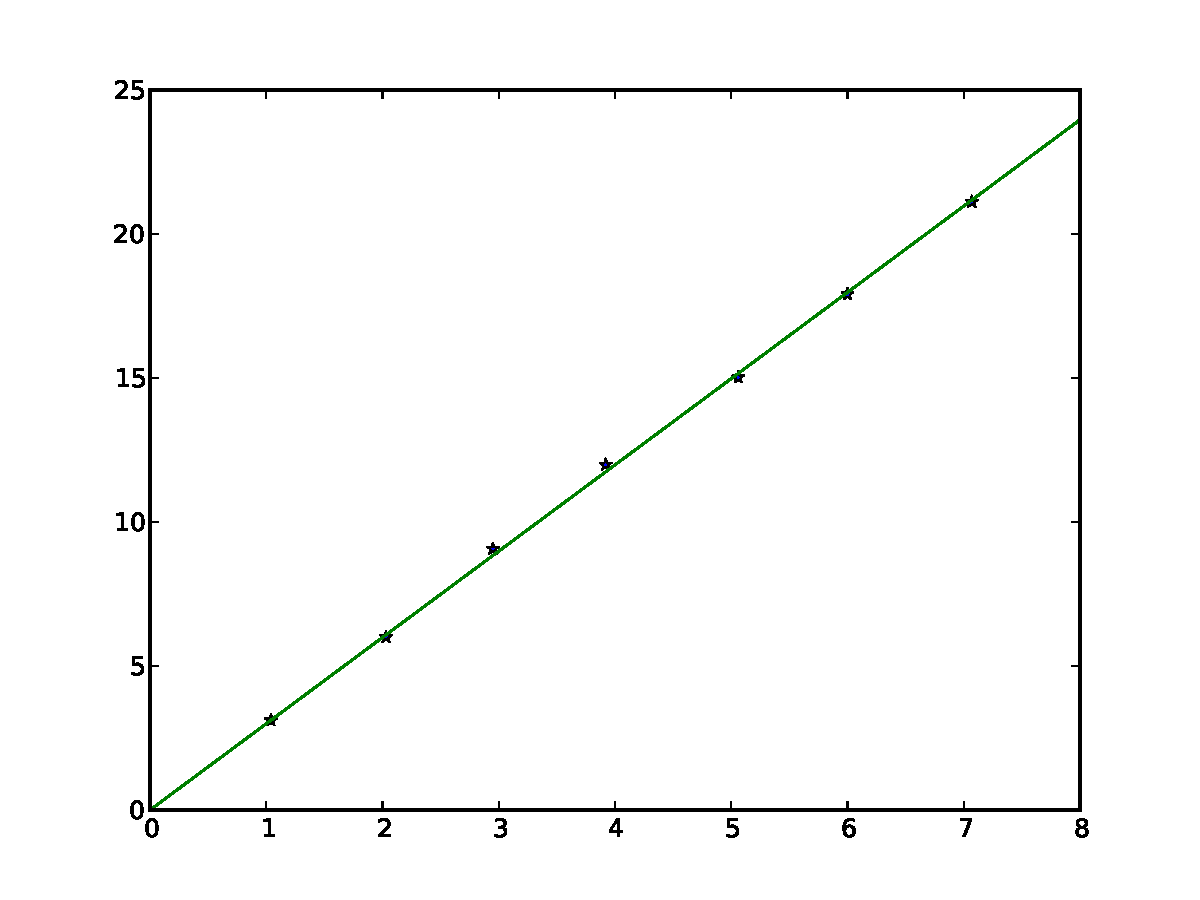
\includegraphics[width=\textwidth]{line_lstsq}
\caption{The graph of the spring data together with its linear fit}
\label{Fig:SpringFit}
\end{center}
\end{figure}

\begin{lstlisting}
>>> from matplotlib import pyplot as plt
>>> x0 = np.linspace(0,8,100)
>>> y0 = k[0]*x0
>>> plt.plot(A,b,'*',x0,y0)
>>> plt.show()
\end{lstlisting}
See Figure \ref{Fig:SpringFit} to see how well the line fits the data.


\section*{General Line Fitting}

Suppose that we wish to fit a general line, that is $y=m x+b$, to the data set 
$\{(x_k,y_k)\}^n_{k=1}$.  Assume that the line does not cross through the origin, 
as in the previous example.  Then we seek both a slope and a $y$-intercept.  
In this case, we set up the following linear system $A x = b$, or more precisely
\[
\begin{pmatrix}
x_1 & 1\\
x_2 & 1\\
x_3 & 1\\
\vdots & \vdots\\
x_n & 1
\end{pmatrix}
\begin{pmatrix}
m\\
b
\end{pmatrix}=
\begin{pmatrix}
y_1\\
y_2\\
y_3\\
\vdots\\
y_n
\end{pmatrix}.
\]
Note that $A$ has rank $2$ as long as not all of the $x_k$ values are the same.  
Hence, the least squares solution
is given by
$$
\widehat{x} = (A^HA)^{-1}A^Hb.
$$
In what sense does this solution give us the best fit line for the data? Recall that since $A$ is injective,
the matrix $A(A^HA)^{-1}A^H$ is an orthogonal projector onto the range of $A$, which means that
$A(A^HA)^{-1}A^Hb = A\widehat{x}$ is the closest vector (with respect to the 2-norm) to $b$ that lies in the
range of $A$. That is, $\widehat{x}$ minimizes the error between $Ax$ and $b$, where the error is given
by the distance between these vectors, $\|b-Ax\|_2$. Another way to say this is that $\widehat{x}$ gives the
values $m$ and $b$ for which the sum of the squares of the distances from each data point $y_k$ to the value
$y = mx_k + b$ is as small as possible.

\section*{Loading Data from .npz Files}
For Least Squares problems as well as in many other contexts, loading data is often a necessary step before
proceeding with further analysis. Here we briefly review another data format in Python and the commands used
to load the data.

A \li{.npz} file is a compressed binary file that contains an archive of NumPy data structures.
A given file may therefore contain several arrays, each array associated with a unique string that identifies it.
When you load a \li{.npz} file in Python, a dictionary-like object is returned, and you can access the data by
providing the appropriate key. Note that when you load a \li{.npz} file, you must also be sure to close it when
you are finished. This is taken care of automatically if you use the \li{with ... as} keywords.

As an example, suppose that we have a file named \li{grades.npz} that contains several arrays, each giving the
homework scores of a particular student in a particular class. Assuming that one of the arrays is associated with
the key \li{'Abe'}, we can load this array in the following way:

\begin{lstlisting}
>>> with np.load('grades.npz') as grades:
>>>     abe_grades = grades['Abe']
>>> abe_grades
array([ 10.,  10.,  10.,  10.,  10.,  10.,  10.,  10.,  10.,  10.])
\end{lstlisting}

You will need to apply this technique in the next problem.

\begin{problem}
Write a function \li{fitLine} that takes no arguments executes the following.
Load the \texttt{linepts} array from \texttt{data.npz}.
This consists of two columns corresponding to the $x$ and $y$ values of a given data set.  
Use least squares to find the slope and $y$-intercept that best fits the data.  
Then plot the data points and the line on the same graph.
The function should not return anything.
\end{problem}

\section*{Fitting data to a circle}

Recall that the equation of a circle, with radius $r$ centered at $(c_1,c_2)$, is given by
\begin{equation}
\label{circle}
(x-c_1)^2 + (y-c_2)^2 = r^2.
\end{equation}
Suppose we are given a set of data points closely forming a circle $\{(x_i,y_i)\}^n_{i=1}$.  
The ``best'' fit is found via least squares by expanding \eqref{circle} to get
\[
2 c_1 x + 2 c_2 y + c_3 = x^2 + y^2,
\]
where $c_3 = r^2 - c_1^2 - c_2^2$.  Then we can write the linear system $A x = b$ as
\[
\begin{pmatrix}
2 x_1 & 2 y_1 & 1\\
2 x_2 & 2 y_2 & 1\\
\vdots & \vdots & \vdots \\
2 x_n & 2 y_n & 1
\end{pmatrix}
\begin{pmatrix}
c_1\\
c_2\\
c_3
\end{pmatrix}=
\begin{pmatrix}
x_1^2 + y_1^2\\
x_2^2 + y_2^2\\
\vdots\\
x_n^2 + y_n^2
\end{pmatrix},
\]
where the matrix $A$ and the vector $b$ are obtained by the given data and the unknown
$x$ contains the information about the center and radius of the circle and is obtained 
by finding the least squares solution.

\section*{Example}

In this section, we fit the following points to a circle:
\begin{align*}
&(134,76),(104,146),(34,176),(-36,146),\\
&(-66,76),(-36,5),(34,-24),(104,5),(134,76)
\end{align*}

We enter them into Python as a $9\times 2$ array:
\begin{lstlisting}
>>> P = np.array([[134,76],[104,146],[34,176],[-36,146],
                  [-66,76],[-36,5],[34,-24],[104,5],[134,76]])
\end{lstlisting}
We compute $A$ and $b$ by entering the following:
\begin{lstlisting}
>>> A = A =np.hstack((2*P, np.ones((9,1))))
>>> b = (P**2).sum(axis=1)
\end{lstlisting}
Hence, we get the least squares solution
\begin{lstlisting}
>>> x = np.dot(np.dot(la.inv(np.dot(A.T,A)),A.T),b)
\end{lstlisting}
Then we find $c_1$, $c_2$, and $r$ by:
\begin{lstlisting}
>>> from math import sqrt
>>> c1, c2, c3 = x
>>> r = sqrt(c1**2 + c2**2 + c3)
\end{lstlisting}
We plot this by executing
\begin{lstlisting}
>>> theta = np.linspace(0,2*np.pi,200)
>>> plt.plot(r*np.cos(theta)+c1,r*np.sin(theta)+c2,'-',P[:,0],P[:,1],'*')
>>> plt.show()
\end{lstlisting}


\begin{problem}
Write a function \li{fitCircle} that does the following.
Load the \texttt{circlepts} array from \texttt{data.npz}.
This consists of two columns corresponding to the $x$ and $y$ values of a given 
data set.  Use least squares to find the center and radius of the circle that best 
fits the data.  Then plot the data points and the circle on the same graph.
The function should return nothing.
\end{problem}

\begin{problem}
The general equation for an ellipse is:
\[
ax^2 + bx + cxy + dy + ey^2 = 1
\]

Write a function \li{fitEllipse} that uses least squares to fit data to an ellipse. 
The function should take a $n\times 2$ array as input, where the first column gives the $x$-coordinates
and the second column gives the $y$-coordinates. Find the least squares solution for $a, b, c, d,$ and $e$,
and return the solution.
\end{problem}

In these Least Squares problems, we have found best fit lines and ellipses relative to the 2-norm.
It is possible to generalize the idea of best fit curves relative to other norms. 
See Figure \ref{Fig:ellipse} for an illustration of this.

\begin{figure}[h]
\label{ellipsefit}
\centering
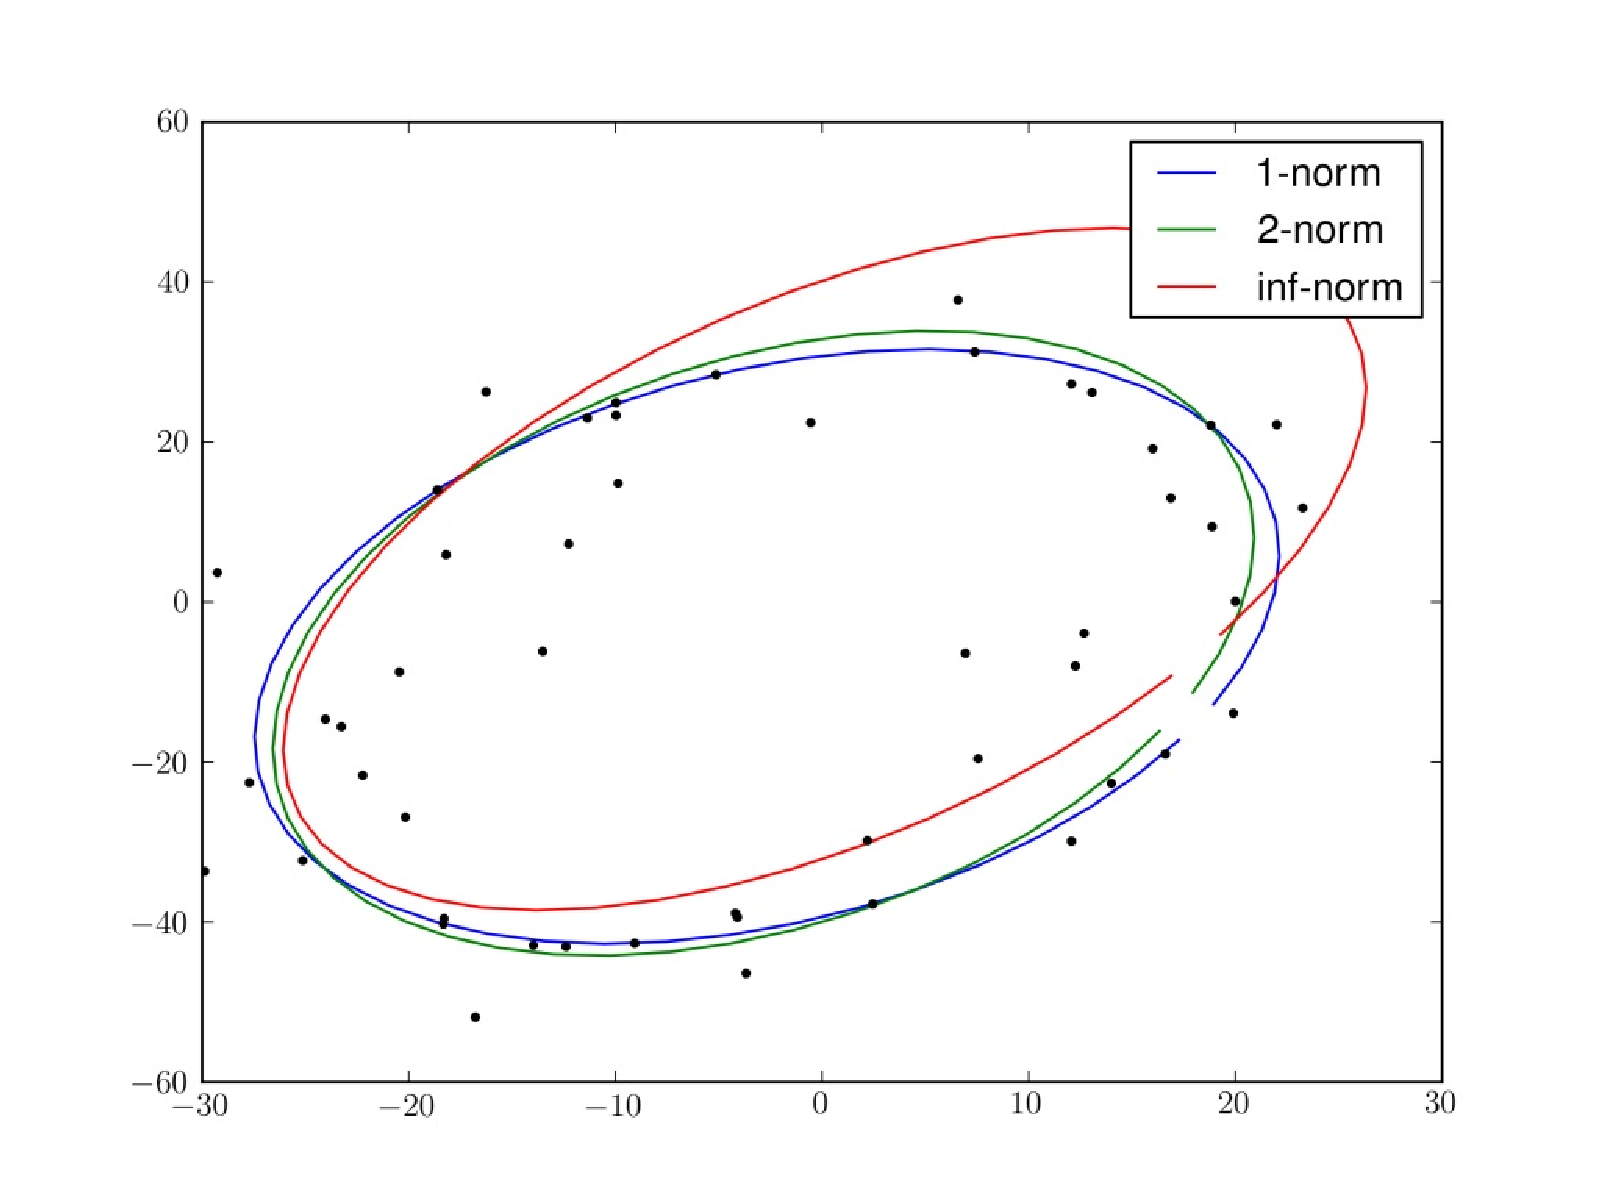
\includegraphics[width=\textwidth]{ellipsefit.pdf}
\caption{Fitting an ellipse using different norms.}
\label{Fig:ellipse}
\end{figure} 